\documentclass[10pt, onecolumn]{article}
\usepackage[margin=1in]{geometry}
\usepackage{lmodern}% http://ctan.org/pkg/lm

% use Unicode characters
% try changing the option if you run into troubles with special characters
% (e.g. umlauts)
\usepackage[utf8x]{inputenc}
% hyperref makes references clicky.
\usepackage{nameref}
% line numbers
\usepackage[right]{lineno}
% improves typesetting in LaTeX
% \usepackage{microtype}
% degree symbol
\usepackage{gensymb}
\usepackage{amsmath}
\usepackage{booktabs}
\usepackage[numbers,super]{natbib}

% use adjustwidth environment to exceed text width (see examples in text)
\usepackage{changepage}

% adjust caption style
\usepackage[aboveskip=1pt,labelfont=bf,
            labelsep=period,singlelinecheck=off]{caption}

% remove brackets from references
\makeatletter
\renewcommand{\@biblabel}[1]{\quad#1.}
\makeatother

\usepackage[colorinlistoftodos]{todonotes}

% headrule, footrule and page numbers
\usepackage{lastpage,fancyhdr,graphicx}
\usepackage{epstopdf}
\pagestyle{myheadings}
\pagestyle{fancy}
\fancyhf{}
\rfoot{\thepage/\pageref{LastPage}}
\renewcommand{\footrule}{\hrule height 2pt \vspace{2mm}}

% use \textcolor{color}{text} for colored text (e.g. highlight to-do areas)
\usepackage{color}

% define custom colors (this one is for figure captions)
\definecolor{Gray}{gray}{.25}

% this is required to include graphics
\usepackage{graphicx}

% use if you want to put caption to the side of the figure - see example in text
\usepackage{sidecap}

% hyperurls packages:
\usepackage{xcolor}
\usepackage[colorlinks = true,
            linkcolor = blue,
            urlcolor  = blue,
            citecolor = blue,
            anchorcolor = blue]{hyperref}


% use for have text wrap around figures
\usepackage{wrapfig}
\usepackage[pscoord]{eso-pic}
\usepackage[fulladjust]{marginnote}
\reversemarginpar{}

% Make figures be labelled as S#
\renewcommand{\thefigure}{S\arabic{figure}}


% new commands
% q value
\newcommand{\qval}[1]{$q<10^{-#1}$}

% species names
\newcommand{\cel}{\emph{C.~elegans}}
\newcommand{\dicty}{\emph{D.~discoideum}}
\newcommand{\ecol}{\emph{E.~coli}}

% gene names
\newcommand{\gene}[1]{\emph{#1}}

\newcommand{\nlp}{\emph{\mbox{nlp-31}}}
\newcommand{\ftna}{\emph{\mbox{ftn-1}}}
\newcommand{\ftnb}{\emph{\mbox{ftn-2}}}
\newcommand{\cysl}{\emph{\mbox{cysl-1}}}
\newcommand{\nog}{\emph{\mbox{nog-1}}}
\newcommand{\nhr}{\emph{\mbox{nhr-57}}}
\newcommand{\lam}{\emph{\mbox{lam-3}}}

\newcommand{\fog}{\emph{\mbox{fog-2(lf)}}}
\newcommand{\egl}{\emph{\mbox{egl-9}(lf)}}
\newcommand{\rhy}{\emph{\mbox{rhy-1}(lf)}}
\newcommand{\vhl}{\emph{\mbox{vhl-1}(lf)}}
\newcommand{\eglvhl}{\emph{\mbox{egl-9(lf);vhl-1(lf)}}}
\newcommand{\eglhif}{\emph{\mbox{egl-9(lf)}~\mbox{hif-1(lf)}}}
\newcommand{\hif}{\emph{\mbox{hif-1(lf)}}}

% protein names
\newcommand{\eglp}{EGL-9}
\newcommand{\rhyp}{RHY-1}
\newcommand{\nogp}{NOG-1}
\newcommand{\vhlp}{VHL-1}
\newcommand{\hifp}{HIF-1}
\newcommand{\fogp}{FOG-2}
\newcommand{\nhrp}{NHR-57}
\newcommand{\lamp}{LAM-3}
\newcommand{\cyslp}{CYSL-1}

% DE genes numbers:
\newcommand{\egln}{2,549}
\newcommand{\rhyn}{3,005}
\newcommand{\vhln}{1,275}
\newcommand{\eglvhln}{3,654}
\newcommand{\hifn}{1,075}
\newcommand{\eglhifn}{744}
\newcommand{\fogn}{2,840}
\newcommand{\total}{7,609}

% downstream targets
\newcommand{\egltargets}{4}
\newcommand{\rhytargets}{0}
\newcommand{\vhltargets}{71} % 72 minus vhl-1 (IDed due to deletion)
\newcommand{\hiftargets}{312}
\newcommand{\hifohtargets}{56}

% website commands
\newcommand{\website}{
            \url{https://wormlabcaltech.github.io/mprsq/}
            }
\newcommand{\webref}{
\href{https://wormlabcaltech.github.io/mprsq/}{website}}

% more space between rows
\newcommand{\ra}[1]{\renewcommand{\arraystretch}{#1}}

\newcommand{\titleone}{Genetic Analysis of a Metazoan Pathway using
Transcriptomic Phenotypes, Supplementary Information}

\title{
  \Large
  \textbf{\titleone}
}

\author{David Angeles-Albores\textsuperscript{1, 2,$\dagger{}$}
\and{}
Carmie Puckett Robinson\textsuperscript{1, 2, 3,$\dagger{}$}
\and{}
Brian A. Williams\textsuperscript{1}
\and{}
Barbara J. Wold\textsuperscript{1}
\and{}
Paul W. Sternberg\textsuperscript{1, 2, *}
}

% document begins here
\begin{document}
\linenumbers{}

% title
\maketitle
% author info
\textbf{$\dagger$} These authors contributed equally to this work\\
\textbf{1} Division of Biology and Biological Engineering, Caltech,
Pasadena, CA, 91125, USA\\
\textbf{2} Howard Hughes Medical Institute, Caltech, Pasadena, CA, 91125, USA\\
\textbf{3} Department of Neurology, Keck School of Medicine, University of
Southern California, Los Angeles, California, 90033, USA\\
\textbf{*} Corresponding author. Contact: pws@caltech.edu


\section*{A quality check of the transcriptomic data reveals excellent agreement
            with the literature}
\label{sub:quality_check}
One way to establish whether genes are acting additively or epistatically to each
other is to perform qPCR of a reporter gene in the single and double mutants. This
approach was used to successfully map the relationships within the hypoxia
pathway (see, for example~\cite{Shao2009,Shen2006}). A commonly used hypoxia reporter
gene is \nhr{}, which is known to exhibit a several-fold increase in mRNA
expression when \hifp{} accumulates~\cite{Shen2006,Shen2005,Park2012}. Likewise,
increased \hifp{} function is known to cause increased transcription of
\gene{rhy-1} and \gene{egl-9}~\cite{Powell-Coffman2010}.

We can
selectively look at the expression of a few genes at a time. Therefore, we
queried the changes in expression of \gene{rhy-1}, \gene{egl-9}, and \nhr{}. We
included the nuclear laminin gene \lam{} as a representative negative control not
believed to be responsive to alterations in the hypoxia pathway.
\nhr{} was upregulated in \egl{}, \rhy{} and \vhl{}, but remains unchanged in \hif{}.
\eglvhl{} had an expression level similar to \egl{}; whereas the
\eglhif{} mutant showed wild-type levels of the reporter expression, as reported
previously~\cite{Shen2006} (see Fig.~\ref{fig:qpcr}).

% in silico qPCR
\begin{figure}[tbhp]
  \centering
  \includegraphics[width=.5\textwidth]{../figs/qpcr.pdf}
  \caption{
    Observed $\beta$ values of select genes. We selected
    four genes (\gene{rhy-1}, \gene{egl-9}, \nhr{} and \lam{}, shown on the x-axis)
    and plotted their regression coefficients, $\beta$, as measured for every
    genotype (represented by one of six colors) to study the epistatic relationships
    between each gene. Asterisks above a bar represent a regression coefficient
    statistically significantly different from 0 (\qval{1}) relative to a wild-type
    control. Error bars show standard error of the mean
    value of $\beta$. \nhr{} is an expression reporter that has been used previously
    to identify \gene{hif-1} regulators~\cite{Shen2006,Shao2009}. \lam{} is shown here
    as a negative control that should not be altered by mutations in this pathway.
    We measured modest increases in the levels of \gene{rhy-1} mRNA when \hif{} is
    knocked out.
}
\label{fig:qpcr}
\end{figure}

We observed changes in \rhy{} expression consistent with previous
literature~\cite{Shen2006} when \hifp{} accumulates.
We also observed increases in \gene{egl-9} expression in \egl{}.
\gene{egl-9} is known as a hypoxia responsive gene~\cite{Powell-Coffman2010}.
Although changes in \gene{egl-9} expression were not statistically significantly
different from the wild-type in
\rhy{} and \vhl{} mutants, the mRNA levels of \gene{egl-9} still trended towards
increased expression in these genotypes.
As with \nhr{}, \gene{egl-9} and \gene{rhy-1} expression were wild-type in
\eglhif{} and \eglvhl{} mutant showed expression phenotypes identical to \egl{}.
This dataset also showed that knockout of \gene{hif-1} resulted in a modest
increase in the levels of \gene{rhy-1}. This suggests that \gene{hif-1}, in
addition to being a positive regulator of \gene{rhy-1} when strongly expressed,
also inhibits \gene{rhy-1}, which constitutes a novel observation.
Using a single reporter we would have been able to reconstruct an
important fraction of the genetic relationships between the genes in the hypoxia
pathway–--but would likely fail to observe yet other genetic interactions, such as
the evidence for \gene{hif-1} negatively regulating \gene{rhy-1} transcript levels.

\section*{Weighted Correlations}
% correlative genetics again
  \begin{figure}[tbhp]
  \centering
  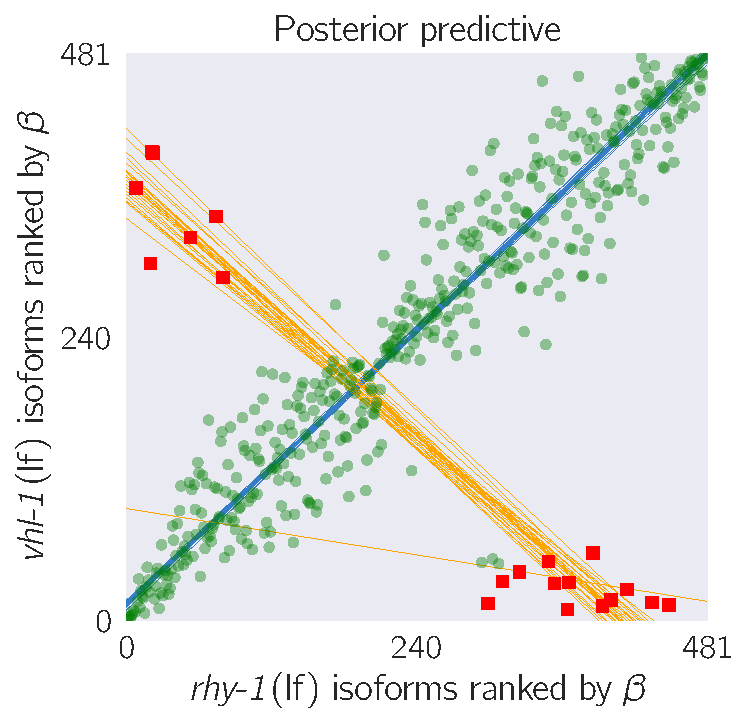
\includegraphics[width=.4\textwidth]{../figs/multiplemodes-ed.pdf}
  \caption{
    A feedback loop can generate transcriptomes that are both
    correlated and anti-correlated. The \vhl{}/\rhy{} STP shows a cross-pattern.
    Green large points are inliers to the first
    regression. Red squares are outliers to the first regression. Only the red
    small points were used for the secondary regression. Blue lines are representative
    samples of the primary bootstrapped regression lines. Orange lines are
    representative samples of the secondary bootstrapped regression lines.
  }
\label{fig:xpattern}
\end{figure}

After we calculated the pairwise correlation within each STP,
we weighted the result of each regression by the
number of isoforms within the STP and
divided by the total number of differentially expressed isoforms present in the
two mutant transcriptomes that contributed to that specific STP,
$N_\mathrm{overlap}/N_{\mathrm{g_1} \cup \mathrm{g2}}$.
The weighted regressions recapitulated a module network (see Fig.~\ref{fig:heatmap}).
We identified a strong positive interaction between \egl{} and \rhy{}.
The magnitude of this weighted correlation derives from the number of genes
that are differentially expressed for these mutants (\egln{} and \rhyn{}
DEGs respectively) and the size of their STP, which makes
the weighting factor considerably larger than other pairs.
The weak correlation between \hif{} and \egl{} results from the large effect size
of the \egl{} transcriptome coupled with the small STP between both mutants.

The fine-grained nature of transcriptional phenotypes means that these weighted
correlations between transcriptomes of single mutants are predictive of genetic
interaction.

% heatmap
\begin{figure}[tbhp]
  \centering
  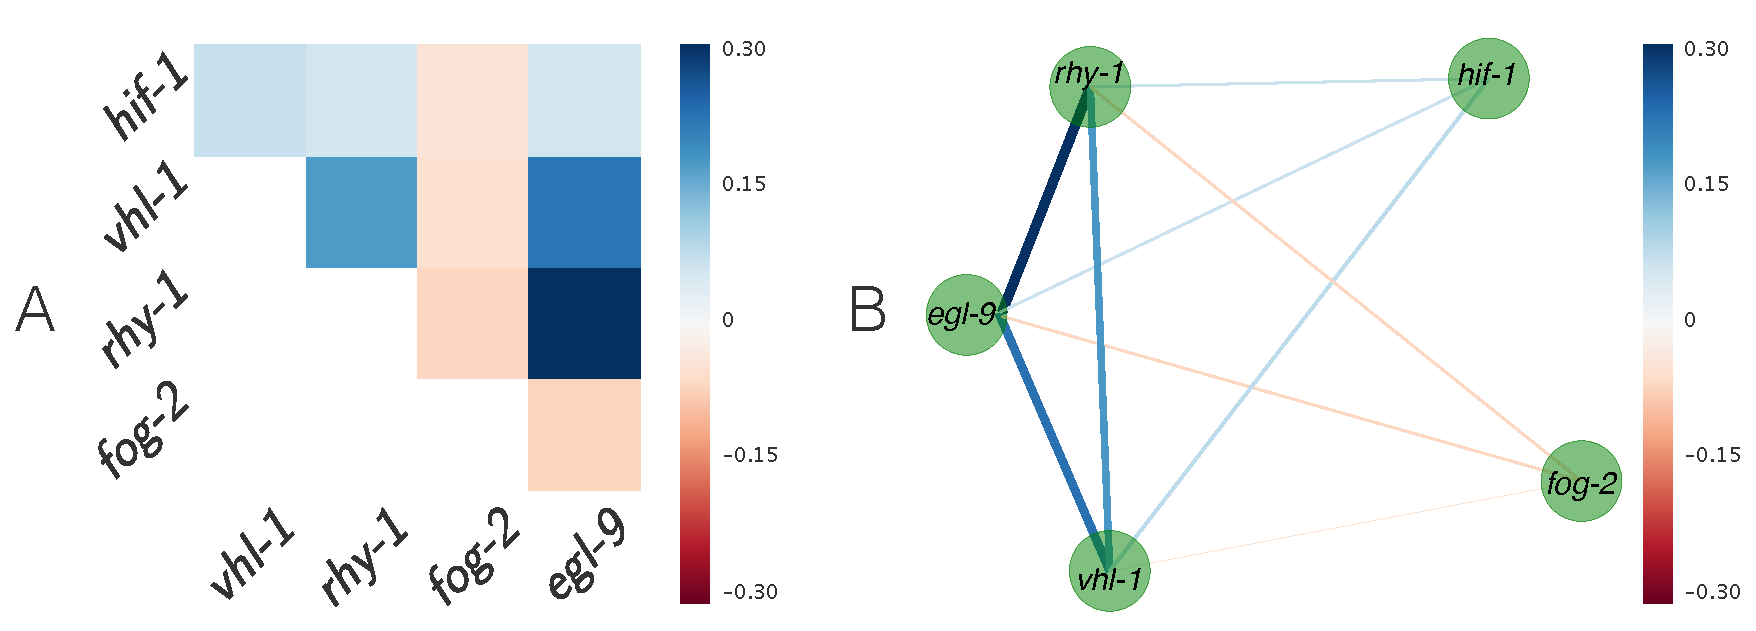
\includegraphics[width=\textwidth]{../figs/bayesian-heatmap-horizontal.pdf}
  \caption{
    \textbf{A}. Heatmap showing pairwise regression values between all
    single mutants. \textbf{B}. Correlation network drawn from \textbf{A}. Edge
    width is proportional to the logarithm of the magnitude of the weighted
    correlation between two nodes divided by absolute value of the weighted
    correlation value of smallest magnitude. Edges are also colored according to the
    heatmap in \textbf{A}. Inhibitors of \gene{hif-1} are tightly correlated and form
    a control module;
    \gene{hif-1} is positively correlated to its inhibitors, albeit weakly;
    and
    \gene{fog-2}, a gene that is not reported to interact with the hypoxia pathway,
    has the smallest, negative correlation to any gene.
}
\label{fig:heatmap}
\end{figure}

\subsubsection*{Enrichment analysis of the hypoxia response}
\label{sub:ea_hypoxia}
To validate that our transcriptomes were correct, and to understand how
biological functions may vary between them, we subjected each decoupled response to
enrichment analysis using the WormBase Enrichment Suite~\cite{Angeles-Albores2016,
Angeles-Albores2016b}.

\begin{figure}[tbhp]
  \centering
  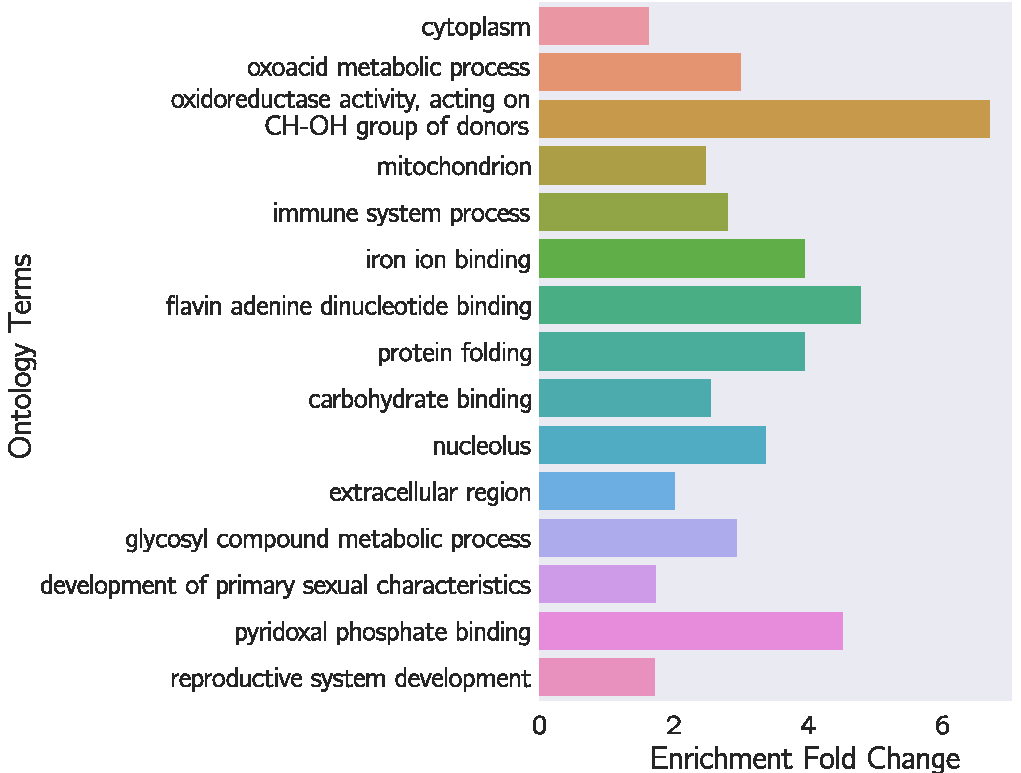
\includegraphics[width=.5\textwidth]{../figs/hypoxia_response_gea.pdf}
  \caption{
    Gene ontology enrichment analysis of genes associated with the main hypoxia response.
    A number of terms reflecting catabolism and bioenergetics are enriched.
  }
\label{fig:hyp_gea}
\end{figure}

We used gene ontology enrichment analysis (GEA) on the main hypoxia response program.
This showed that the terms `oxoacid metabolic process' (\qval{4}, 3.0 fold-enrichment,
24 genes), `iron ion binding' (\qval{2}, 3.8 fold-enrichment, 10 genes), and `immune
system process' (\qval{3}, 2.9 fold-enrichment, 20 genes) were significantly enriched.
GEA also showed enrichment of the term `mitochondrion' (\qval{3}, 2.5 fold-enrichment,
29 genes) (see Fig.~\ref{fig:hyp_gea}). Indeed, \hif{} has been implicated in
all of these biological and molecular functions~\cite{Luhachack2012,Ackerman2012,
Romney2011,Semenza2011}.
As benchmark on the quality of our data, we selected a set of 22 genes known to
be responsive to \hifp{} levels from the literature and asked whether these genes
were present in our hypoxia response list. We found $8/22$ known genes, which
constitutes a statistically significant result ($p<10^{10}$). The small number of
reporters found in this list probably reflects the conservative nature of our
estimates.
We studied the \gene{hif-1}-independent, \gene{vhl-1}-dependent gene set
using enrichment analysis but no terms were significantly enriched.

\subsection*{\hifp{} in the cellular context}
\label{sub:metabolism}

We identified the transcriptional changes
associated with bioenergetic pathways in \cel{} by extracting from
WormBase all genes associated with the tricarboxylic acid (TCA) cycle, the
electron transport chain (ETC) and with the \cel{} GO term energy reserve.
Previous research has described the effects of mitochondrial dysfunction in
eliciting the hypoxia response~\cite{Lee2010}, but transcriptional control
of bioenergetic pathways by \hifp{} has not been studied as extensively in \cel{}
as in vertebrates (see, for example~\cite{Semenza1994,Semenza2012}).
We also searched for the changes in ribosomal components and the proteasome, as
well as for terms relating to immune response (see Fig~\ref{fig:genomewide}).

\begin{figure}[tbhp]
\centering
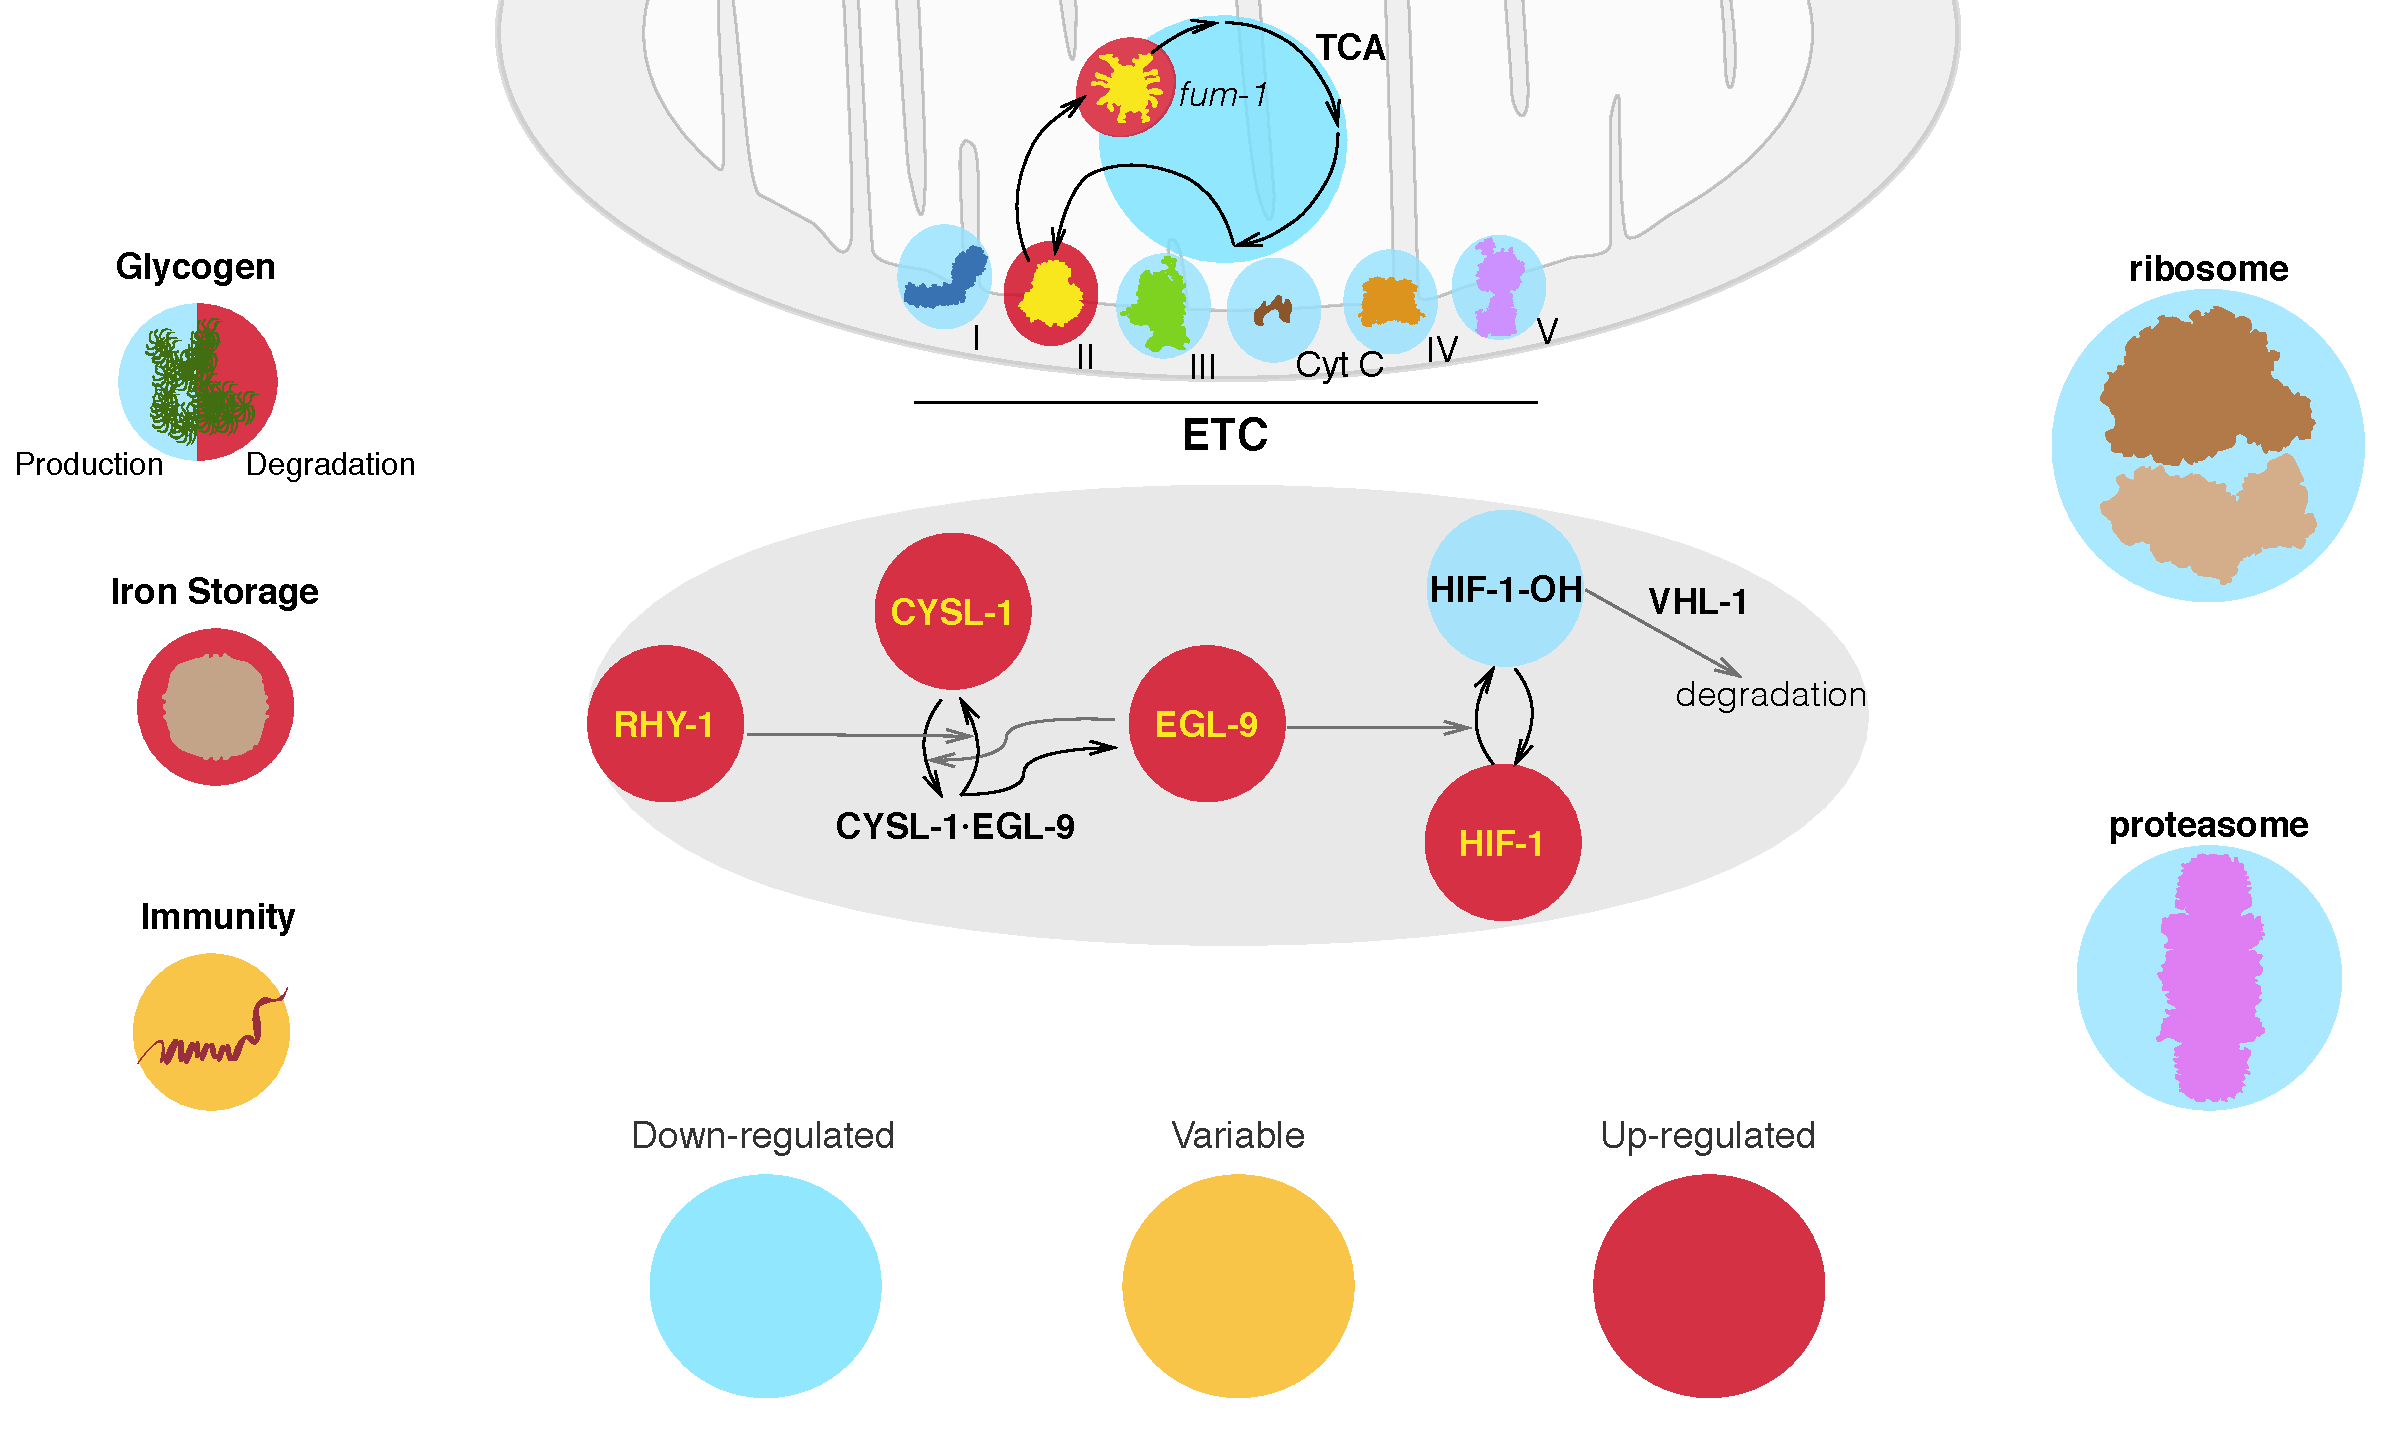
\includegraphics[width=.7\textwidth]{../figs/hif1genomewide.pdf}
\caption{
A graphic summary of the genome-wide effects of \hifp{} from our RNA-seq data.
}
\label{fig:genomewide}
\end{figure}

\subsubsection*{Bioenergetic pathways}
Our data shows that most of the enzymes involved in the TCA cycle and in the ETC
are down-regulated when \hifp{} is induced in agreement with the previous
literature~\cite{Semenza2012}.
However, the fumarase gene \gene{fum-1} and the mitochondrial complex II stood out
as notable exceptions to the trend, as they were up-regulated in every single
genotype that causes deployment of the hypoxia response. FUM-1 catalyzes the
reaction of fumarate into malate, and complex II catalyzes the reaction of
succinate into fumarate. Complex II has been identified as a source of reserve
respiratory capacity in neonatal rat cardiomyocytes previously~\cite{Pfleger2015}.
We found two energy reserve genes that were down-regulated by \hifp{}.
\gene{aagr-1} and \gene{aagr-2}, which are predicted to function in glycogen
catabolism~\cite{Sikora2010}.
Three distinct genes involved in energy reserve were up-regulated. These genes were
\gene{ogt-1}, which encodes O-linked GlcNac Transferase gene; \gene{T04A8.7},
encoding an ortholog of human glucosidase, acid beta (GBA); and \gene{T22F3.3},
encoding ortholog of human glycogen phosphorylase isozyme in the muscle (PYGM).

\subsubsection*{Protein synthesis and degradation}
\hif{} is also known to inhibit protein synthesis and translation in varied
ways.~\cite{Brugarolas2004}. Most reported effects of
\hifp{} on the translation machinery are posttranslational, and no reports to date
show transcriptional control of the ribosomal machinery in \cel{} by \hifp{}. We
used the WormBase Enrichment Suite Gene Ontology
dictionary~\cite{Angeles-Albores2016b} to extract 143 protein-coding genes
annotated as `structural constituents of the ribosome' and we queried whether
they were differentially expressed in our mutants. \egl{}, \vhl{}, \rhy{} and
\egl{};\vhl{} showed differential expression of 91 distinct ribosomal constituents
(not all constituents were detected in all genotypes). For every one of these
genotypes, these genes were always down-regulated. In contrast, \hif{} showed
up-regulation of a single ribosomal constituent.

Next, we asked whether \hifp{} has any transcriptional effects on the
proteasomal constituents; no such effects of \hifp{} on the proteasome
have been reported in \cel{}. Out of 40 WormBase-annotated proteasomal constituents,
we found 31 constituents whose genes were downregulated in at least two out of
the four genotypes we studied. Every gene we found was down-regulated
in at least two out of the four genotypes we studied.

\subsection*{A cellular view of hypoxia}
In addition to reconstructing the pathway, our dataset allowed us
to observe a wide variety of physiologic changes that occur as a result of the
\hifp{}-dependent hypoxia response. In particular, we observed down-regulation of most
components of the TCA cycle and the mitochondrial electron transport chain with
the exceptions of \gene{fum-1} and the mitochondrial complex II.\@The mitochondrial
complex II catalyzes the reaction of succinate into fumarate.
In mouse embryonic fibroblasts, fumarate has been
shown to antagonize \hifp{} prolyl hydroxylase domain (PHD) enzymes, which are
orthologs of \eglp{}~\cite{Sudarshan2009}.
If the inhibitory role of fumarate on PHD enzymes is conserved in \cel{},
upregulation of complex II by \hifp{} during hypoxia may increase
intracellular levels of fumarate, which in turn could lead to elevated
levels of \hifp{}
even after normoxia resumes. The increase in fumarate produced by the complex
could be compensated by increasing expression of \gene{fum-1}. Increased fumarate
degradation allows \cel{} to maintain plasticity in the hypoxia pathway, keeping
the pathway sensitive to oxygen levels.


%This is where your bibliography is generated.
\bibliography{citations}

%This defines the bibliographies style.
\bibliographystyle{naturemag}

\end{document}
